% ===================== MemTrace / MemTraceBench =====================
\subsection{MemTrace (MemTraceBench)}\label{ds:memtrace}
\naturalbadge\ \okbadge\ \lbl{operation + error type}\ \lbl{memory system (single-agent)}\ \lbl{LoCoMo / LongMemEval / RealMem}

\begin{identity}
Paper & \emph{MemTrace: Tracing and Attributing Errors in Large Language Model Memory Systems} --- Deng et al.\ (Zhejiang University, ZJUNLP, 18 authors), arXiv:2605.28732, May 2026 (v4 Oct 2026, marked ``ongoing work'') \cite{memtrace2026}\\
Links & \href{https://huggingface.co/datasets/zjunlp/MemTraceBench}{HF \code{zjunlp/MemTraceBench}} \textperiodcentered\ \href{https://github.com/zjunlp/MemTrace}{GitHub \code{zjunlp/MemTrace}} \textperiodcentered\ graph tooling \href{https://github.com/zjunlp/MemBase}{\code{zjunlp/MemBase}} / \href{https://github.com/zjunlp/smartcomment}{\code{zjunlp/smartcomment}}\\
License & MIT (dataset card, code and paper); source conversations from LoCoMo, LongMemEval, RealMem\\
Status & downloaded in full, ungated; 6.0 GB; \code{data/memtrace/\{rag,mem0,evermemos,long\_context\}/*.json} (103 execution graphs, 6.6 MB -- 532 MB each)\\
\end{identity}

\begin{multicols}{2}
\paragraph{Description} MemTrace moves failure attribution from the planner/tool loop into the \emph{memory system}. A memory pipeline (extraction $\to$ update/delete $\to$ retrieval $\to$ answer) is instrumented so that each run becomes an \emph{execution graph}: a bipartite DAG of variable nodes (messages, extracted facts, memory units, retrieved sets, prompts, predictions) and operation nodes (extraction, update, deletion, retrieval, filtering, judging, answering) joined by information-flow edges. Given a failed query (prediction $\neq$ gold), the task is to name the \emph{earliest decisive faulty operation} $o^*$ and its error type. Four systems were run with GPT-4.1-mini (Claude Opus 4.5 as answer judge) on three multi-session memory-QA sets (LoCoMo, LongMemEval, RealMem):
\begin{itemize}
\item \textbf{Long-Context} (whole history in the prompt), \textbf{Naive RAG}, \textbf{Mem0}, \textbf{EverMemOS} (Qwen3-Embedding-4B / Reranker-4B).
\end{itemize}
Failures are natural: 1,514 judged-wrong answers were collected (RAG 467, Long-Context 279, Mem0 466, EverMemOS 302) and annotated until 40 \emph{system-caused} failures per system were confirmed. \textbf{Annotation}: five annotators from the author team, a $>$10-page guideline and a Streamlit UI; each case gets three independent labels, then majority vote and discussion. Annotators first rule out \emph{annotation errors} (gold not supported by the conversation) and \emph{judge errors} (answer actually acceptable), then locate the earliest decisive operation, its cause and type. Pairwise disagreement 3--46\%; no $\kappa$ reported. The released \code{reason} is the human rationale aggregated and polished by GPT-5.5. \textbf{Taxonomy} (7 types): Annotation Error, LLM-as-a-Judge Error, Extraction Error (critical fact never enters memory), Update Error (a later update removes/degrades it), Deletion Error (unit explicitly deleted; 0 cases), Retrieval Error (stored but not retrieved), Response Error (context complete, answer still wrong). There are no agent roles; the operation category (extraction / update / retrieval / evaluation) plays the role of the faulty component.

\paragraph{Metrics and baselines} \textbf{ETA} (error-type accuracy) and \textbf{OIA} (operation-identification accuracy, exact \code{op\_id}) over the 160 cases, plus token cost. The proposed attributor walks operation sub-graphs backwards from the prediction (OBS = observation-only variant). Paper Table 1 (\%):

\begin{center}\small
\begin{tabular}{@{}llcc@{}}\toprule
Backbone & Method & ETA & OIA\\\midrule
GPT-4.1-mini & All-at-Once & 31.9 & 13.1\\
GPT-4.1-mini & MemTrace & 36.5 & 14.2\\
GPT-5.4 & All-at-Once & 51.9 & 18.8\\
GPT-5.4 & MemTrace-OBS & 53.8 & \textbf{46.3}\\
GPT-5.4 & MemTrace & \textbf{54.4} & 38.1\\\bottomrule
\end{tabular}
\end{center}
Per system (GPT-5.4, OBS OIA): RAG 87.5, Mem0 55.0, EverMemOS 35.0, Long-Context 7.5 --- localisation collapses when all evidence sits in one giant prompt. Attribution signals used to rewrite Mem0 prompts raised LoCoMo accuracy by up to 7.62 points.

\paragraph{Schema} One file per (system, conversation), named \code{<split>/} \code{<source>\_<conv-id>.json}: a serialised \code{smartcomment} graph with \code{graph\_id}, \code{metadata} (\code{memtracebench\_system}, \code{memtracebench\_dataset\_source}) and \code{data} holding five lists: \code{nodes} (\code{full\_node\_id} = \code{name@version}, \code{category}, \code{value}, \code{comment}, source \code{filename}/\code{lineno}), \code{operations} (\code{op\_id}, \code{op\_name} such as \code{memory\_system.extract\_facts}, \code{update\_memory\_decision}, \code{search\_vector\_store}, \code{agentic\_final\_rerank}, \code{question-answering}; \code{category}), \code{edges} (\code{source\_full\_node\_id} $\to$ \code{target\_full\_node\_id}, producing \code{op\_id}), \code{sessions}, and \code{annotations} (\code{query}, \code{golden\_answers}, \code{prediction\_id}, \code{source\_evidence(\_ids)}, \code{final\_error\_type}, \code{final\_op\_id}, \code{reason}). No trajectory is stored explicitly: we materialise it as the backward dependency slice of \code{prediction\_id} through \code{edges}, in chronological order.
\end{multicols}

\paragraph{Statistics} computed from the downloaded data (slice = operations feeding the prediction).\par\nobreak\vspace{1pt}
\noindent\begin{minipage}[t]{0.56\linewidth}\vspace{0pt}\small\setlength{\tabcolsep}{4pt}
\begin{tabular}{@{}lrrrrr@{}}\toprule
 & All & RAG & Mem0 & EverM. & LongCtx\\\midrule
execution graphs & 103 & 30 & 19 & 20 & 34\\
memory failures (annot.) & 160 & 40 & 40 & 40 & 40\\
Retrieval / Response err. & 76 / 34 & 37 / 3 & 14 / 1 & 25 / 14 & 0 / 16\\
Update / Extraction err. & 31 / 19 & 0 / 0 & 7 / 18 & 0 / 1 & 24 / 0\\
operations / graph: median & 743 & 630 & 1,009 & 1,407 & 498\\
slice steps / failure: median & 497 & 495 & 81 & 1,447 & 497\\\bottomrule
\end{tabular}

\smallskip Plus 75 Annotation-Error (67 unique queries) and 3 Judge-Error annotations kept in the files (238 in total). By source: LongMemEval 70, LoCoMo 58, RealMem 32 failures (graphs 75 / 16 / 12). Graphs hold on average 3,010 nodes and 5,322 edges (max 17,753 / 32,616); operations per graph 422 -- 4,571. Slice length: mean 805, min 12, max 3,661 operations. The faulty operation lies inside the slice in 140 / 160 cases (misses are mostly Mem0 extraction errors: the fact never became a memory unit, so no edge reaches the prediction); its relative position in the slice is late (mean 0.79, median 0.90) and mean 0.69 among all operations of the graph. Node text per graph: median 20.9\,M characters; per slice median 7.6\,M (Mem0 slices 0.1--0.3\,M).
\end{minipage}\hfill
\begin{minipage}[t]{0.42\linewidth}\vspace{0pt}
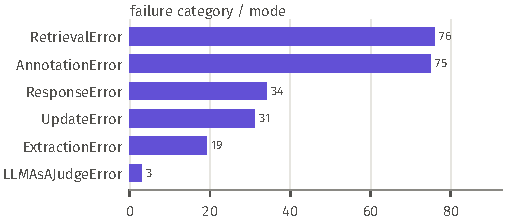
\includegraphics[width=\linewidth]{figures/cat_memtrace.pdf}
\end{minipage}

\paragraph{Example trajectory} \code{mem0/longmemeval\_longmemeval-f8c5f88b.json}, annotation \code{query:f8c5f88b@1} (Mem0 on LongMemEval; Update Error). The prediction's backward slice has 16 operations out of 977 in the graph; at operation 12 an update rewrites ``new tennis racket from a sports store downtown'' into ``focusing on improving tennis game with a new racket'', so retrieval and answering (steps 15--16) no longer see the purchase location. Prompt-template inputs (4--8\,k characters each) are omitted from the rendering.
% auto-generated by scripts/render_traj.py -- do not edit
\trajtask{mem0/\allowbreak{}longmemeval\_longmemeval-f8c5f88b.json:\allowbreak{}:\allowbreak{}query:\allowbreak{}f8c5f88b@1}{'Where did I buy my new tennis racket from?\allowbreak{}'}
\begin{trajstep}{1}{extraction operation (memory\_system.extract\_facts)}{agA}
Operation:\allowbreak{} memory\_system.extract\_facts [extraction] (op\_id op-033d2905d9bf40fd89e86af67a91bb4f,\allowbreak{} session 1ede478b,\allowbreak{} 2026-04-27 01:\allowbreak{}00:\allowbreak{}46.385)\newline Description:\allowbreak{} Extract facts from a conversation snippet using an LLM. Please note that these extracted facts are initially without timestamps,\allowbreak{} which will be added later when the memory unit is created or updated.\newline Inputs:\allowbreak{}\newline - [prompt] fact-extraction-system-prompt (prompt template,\allowbreak{} 4248 chars,\allowbreak{} omitted)\newline - [llm\_response] str:\allowbreak{}c4d3eefad6ce7d259347218d38832b914cd1dff9:\allowbreak{} '\{"facts" :\allowbreak{} ["Planning to check out West Elm and Crate \& Barrel online",\allowbreak{} "Looking to buy new rugs for the living room",\allowbreak{} "Interested in stores\newline [...] (1,\allowbreak{}163 chars omitted) [...]\newline of rugs"]\}'\newline - [llm\_response] str:\allowbreak{}c4d3eefad6ce7d259347218d38832b914cd1dff9:\allowbreak{} '\{"facts" :\allowbreak{} ["Planning to check out West Elm and Crate \& Barrel online",\allowbreak{} "Looking to buy new rugs for the living room",\allowbreak{} "Interested in stores with a wide selection of rugs"]\}'
\end{trajstep}
\begin{trajstep}{2}{update operation (memory\_system.update\_memory\_decision)}{agB}
Operation:\allowbreak{} memory\_system.update\_memory\_decision [update] (op\_id op-35263efef0ab46f3a35b16a39b81dc9b,\allowbreak{} session 1ede478b,\allowbreak{} 2026-04-27 01:\allowbreak{}00:\allowbreak{}47.464)\newline Description:\allowbreak{} Decide how to update the memory store using a large language model.\newline Inputs:\allowbreak{}\newline - [similar\_memories] str:\allowbreak{}3a82ed585fc1d5dae6573a915a7c5fc982cc2b24:\allowbreak{} 'Find 8 existing memories similar to the new extracted facts.'\newline - [llm\_response] str:\allowbreak{}c4d3eefad6ce7d259347218d38832b914cd1dff9:\allowbreak{} ['Planning to check out West Elm and Crate \& Barrel online',\allowbreak{} 'Looking to buy new rugs for the living room',\allowbreak{} 'Interested in stores with a wide selection of rugs']\newline - [prompt] memory-update-decision-prompt (prompt templ\newline [...] (5,\allowbreak{}190 chars omitted) [...]\newline "Likes trendy clothes from Old Navy" \},\allowbreak{} \{ "event":\allowbreak{} "NONE",\allowbreak{} "id":\allowbreak{} "3",\allowbreak{} "text":\allowbreak{} "Planning to buy the Tab S8" \},\allowbreak{} \{ "event":\allowbreak{} "NONE",\allowbreak{} "id":\allowbreak{} "4",\allowbreak{} "te [...]
\end{trajstep}
\begin{trajstep}{3}{extraction operation (memory\_system.extract\_facts)}{agA}
Operation:\allowbreak{} memory\_system.extract\_facts [extraction] (op\_id op-34a8949827c94ee69a40754fcf28a700,\allowbreak{} session 66c23110\_1,\allowbreak{} 2026-04-27 01:\allowbreak{}06:\allowbreak{}01.751)\newline Description:\allowbreak{} Extract facts from a conversation snippet using an LLM. Please note that these extracted facts are initially without timestamps,\allowbreak{} which will be added later when the memory unit is created or updated.\newline Inputs:\allowbreak{}\newline - [prompt] fact-extraction-system-prompt (prompt template,\allowbreak{} 4248 chars,\allowbreak{} omitted)\newline - [llm\_response] str:\allowbreak{}29308fffce86ada19dac92c57e7c41c3554d3b29:\allowbreak{} '\{"facts":\allowbreak{} ["Recently bought an eyeshadow palette at Sephora",\allowbreak{} "Has 200 points in Sephora loyalty program"]\}'\newline - [message] longmemeval-mess\newline [...] (916 chars omitted) [...]\newline eyeshadow palette at Sephora",\allowbreak{} "Has 200 points in Sephora loyalty program"]\}'\newline - [llm\_response] str:\allowbreak{}29308fffce86ada19dac92c57e7c41c3554d3b29:\allowbreak{} '\{"facts":\allowbreak{} ["Recently bought an eyeshadow palette at Sephora",\allowbreak{} "Has 200 points in Sephora loyalty program"]\}'
\end{trajstep}
\begin{trajstep}{4}{update operation (memory\_system.update\_memory\_decision)}{agB}
Operation:\allowbreak{} memory\_system.update\_memory\_decision [update] (op\_id op-46e0d327c91d4e4b85f699f003f7e760,\allowbreak{} session 66c23110\_1,\allowbreak{} 2026-04-27 01:\allowbreak{}06:\allowbreak{}02.721)\newline Description:\allowbreak{} Decide how to update the memory store using a large language model.\newline Inputs:\allowbreak{}\newline - [similar\_memories] str:\allowbreak{}d70b5f680e2b5fcaa09f935df5ebd0d3c31ac49a:\allowbreak{} 'Find 6 existing memories similar to the new extracted facts.'\newline - [llm\_response] str:\allowbreak{}29308fffce86ada19dac92c57e7c41c3554d3b29:\allowbreak{} ['Recently bought an eyeshadow palette at Sephora',\allowbreak{} 'Has 200 points in Sephora loyalty program']\newline - [prompt] memory-update-decision-prompt (prompt template,\allowbreak{} 5460 chars,\allowbreak{} omitted)\newline - [llm\_response] str:\allowbreak{}b06ab983522543\newline [...] (4,\allowbreak{}886 chars omitted) [...]\newline \{ "event":\allowbreak{} "NONE",\allowbreak{} "id":\allowbreak{} "3",\allowbreak{} "text":\allowbreak{} "Had a luxury shopping spree at Neiman Marcus about six weeks ago" \},\allowbreak{} \{ "event":\allowbreak{} "NONE",\allowbreak{} "id":\allowbreak{} "4",\allowbreak{} "text":\allowbreak{} "Open to t [...]
\end{trajstep}
\begin{trajstep}{5}{extraction operation (memory\_system.extract\_facts)}{agA}
Operation:\allowbreak{} memory\_system.extract\_facts [extraction] (op\_id op-21161dcfcdb74761af8361564a97a46b,\allowbreak{} session answer\_c3567066,\allowbreak{} 2026-04-27 01:\allowbreak{}08:\allowbreak{}59.593)\newline Description:\allowbreak{} Extract facts from a conversation snippet using an LLM. Please note that these extracted facts are initially without timestamps,\allowbreak{} which will be added later when the memory unit is created or updated.\newline Inputs:\allowbreak{}\newline - [prompt] fact-extraction-system-prompt (prompt template,\allowbreak{} 4248 chars,\allowbreak{} omitted)\newline - [llm\_response] str:\allowbreak{}738f1c9c10461810e7fd840a33e04a0fab59798f:\allowbreak{} '\{"facts" :\allowbreak{} ["Plays tennis",\allowbreak{} "Has a new tennis racket from a sports store downtown",\allowbreak{} "Feels the new tennis racket has improved their ga\newline [...] (1,\allowbreak{}323 chars omitted) [...]\newline - [llm\_response] str:\allowbreak{}738f1c9c10461810e7fd840a33e04a0fab59798f:\allowbreak{} '\{"facts" :\allowbreak{} ["Plays tennis",\allowbreak{} "Has a new tennis racket from a sports store downtown",\allowbreak{} "Feels the new tennis racket has improved their game",\allowbreak{} "Plans to do exercises before playing tennis"]\}'
\end{trajstep}
\begin{trajstep}{6}{update operation (memory\_system.update\_memory\_decision)}{agB}
Operation:\allowbreak{} memory\_system.update\_memory\_decision [update] (op\_id op-aa7aeb57455146c4965ef8be3f73a5d2,\allowbreak{} session answer\_c3567066,\allowbreak{} 2026-04-27 01:\allowbreak{}09:\allowbreak{}00.594)\newline Description:\allowbreak{} Decide how to update the memory store using a large language model.\newline Inputs:\allowbreak{}\newline - [similar\_memories] str:\allowbreak{}70bc8a22ac4325bb28717881ebf51672a1c1c0f8:\allowbreak{} 'Find 13 existing memories similar to the new extracted facts.'\newline - [llm\_response] str:\allowbreak{}738f1c9c10461810e7fd840a33e04a0fab59798f:\allowbreak{} ['Plays tennis',\allowbreak{} 'Has a new tennis racket from a sports store downtown',\allowbreak{} 'Feels the new tennis racket has improved their game',\allowbreak{} 'Plans to do exercises before playing tennis']\newline - [memory\_entry] memory-unit-0d52\newline [...] (5,\allowbreak{}882 chars omitted) [...]\newline "event":\allowbreak{} "NONE",\allowbreak{} "id":\allowbreak{} "2",\allowbreak{} "text":\allowbreak{} "Wakes up at 6:\allowbreak{}30 AM" \},\allowbreak{} \{ "event":\allowbreak{} "NONE",\allowbreak{} "id":\allowbreak{} "3",\allowbreak{} "text":\allowbreak{} "Has a meeting at 7:\allowbreak{}30 AM" \},\allowbreak{} \{ "event":\allowbreak{} "NON [...]
\end{trajstep}
\begin{trajstep}{7}{extraction operation (memory\_system.extract\_facts)}{agA}
Operation:\allowbreak{} memory\_system.extract\_facts [extraction] (op\_id op-1469467aa52c41b9bc07e27acda865a2,\allowbreak{} session answer\_c3567066,\allowbreak{} 2026-04-27 01:\allowbreak{}09:\allowbreak{}08.319)\newline Description:\allowbreak{} Extract facts from a conversation snippet using an LLM. Please note that these extracted facts are initially without timestamps,\allowbreak{} which will be added later when the memory unit is created or updated.\newline Inputs:\allowbreak{}\newline - [prompt] fact-extraction-system-prompt (prompt template,\allowbreak{} 4248 chars,\allowbreak{} omitted)\newline - [llm\_response] str:\allowbreak{}3200421f4d4a3bea2c9baba6dd7a629cc78bb374:\allowbreak{} '\{"facts" :\allowbreak{} ["Planning to buy new tennis balls this weekend",\allowbreak{} "Is a recreational tennis player"]\}'\newline - [message] longmemeval-message-10\newline [...] (739 chars omitted) [...]\newline :\allowbreak{} ["Planning to buy new tennis balls this weekend",\allowbreak{} "Is a recreational tennis player"]\}'\newline - [llm\_response] str:\allowbreak{}3200421f4d4a3bea2c9baba6dd7a629cc78bb374:\allowbreak{} '\{"facts" :\allowbreak{} ["Planning to buy new tennis balls this weekend",\allowbreak{} "Is a recreational tennis player"]\}'
\end{trajstep}
\begin{trajstep}{8}{update operation (memory\_system.update\_memory\_decision)}{agB}
Operation:\allowbreak{} memory\_system.update\_memory\_decision [update] (op\_id op-99c97880413a4eff81057aa93ebc6a81,\allowbreak{} session answer\_c3567066,\allowbreak{} 2026-04-27 01:\allowbreak{}09:\allowbreak{}09.181)\newline Description:\allowbreak{} Decide how to update the memory store using a large language model.\newline Inputs:\allowbreak{}\newline - [similar\_memories] str:\allowbreak{}d70b5f680e2b5fcaa09f935df5ebd0d3c31ac49a:\allowbreak{} 'Find 6 existing memories similar to the new extracted facts.'\newline - [llm\_response] str:\allowbreak{}3200421f4d4a3bea2c9baba6dd7a629cc78bb374:\allowbreak{} ['Planning to buy new tennis balls this weekend',\allowbreak{} 'Is a recreational tennis player']\newline - [memory\_entry] memory-unit-190e1a18-a552-4b1c-95e4-674e10cc00d6:\allowbreak{} \{ "id":\allowbreak{} "190e1a18-a552-4b1c-95e4-674e10cc00d6",\allowbreak{} "\newline [...] (5,\allowbreak{}251 chars omitted) [...]\newline ay" \},\allowbreak{} \{ "event":\allowbreak{} "UPDATE",\allowbreak{} "id":\allowbreak{} "3",\allowbreak{} "old\_memory":\allowbreak{} "Plays tennis",\allowbreak{} "text":\allowbreak{} "Plays tennis" \},\allowbreak{} \{ "event":\allowbreak{} "NONE",\allowbreak{} "id":\allowbreak{} "4",\allowbreak{} "text":\allowbreak{} [...]
\end{trajstep}
\begin{trajstep}{9}{extraction operation (memory\_system.extract\_facts)}{agA}
Operation:\allowbreak{} memory\_system.extract\_facts [extraction] (op\_id op-5d3029ffb1e749e5bba7b5682f17e7e3,\allowbreak{} session answer\_c3567066,\allowbreak{} 2026-04-27 01:\allowbreak{}09:\allowbreak{}14.042)\newline Description:\allowbreak{} Extract facts from a conversation snippet using an LLM. Please note that these extracted facts are initially without timestamps,\allowbreak{} which will be added later when the memory unit is created or updated.\newline Inputs:\allowbreak{}\newline - [prompt] fact-extraction-system-prompt (prompt template,\allowbreak{} 4248 chars,\allowbreak{} omitted)\newline - [llm\_response] str:\allowbreak{}4f1fe3d732d310c2444187e0546e729f86020aff:\allowbreak{} '\{"facts":\allowbreak{} ["Considering getting a tennis ball machine to practice shots"]\}'\newline - [message] longmemeval-message-10-28-9:\allowbreak{} \{ "content"\newline [...] (616 chars omitted) [...]\newline 32d310c2444187e0546e729f86020aff:\allowbreak{} '\{"facts":\allowbreak{} ["Considering getting a tennis ball machine to practice shots"]\}'\newline - [llm\_response] str:\allowbreak{}4f1fe3d732d310c2444187e0546e729f86020aff:\allowbreak{} '\{"facts":\allowbreak{} ["Considering getting a tennis ball machine to practice shots"]\}'
\end{trajstep}
\begin{trajstep}{10}{update operation (memory\_system.update\_memory\_decision)}{agB}
Operation:\allowbreak{} memory\_system.update\_memory\_decision [update] (op\_id op-c3a40398534a4d0f9509c706c588b4c8,\allowbreak{} session answer\_c3567066,\allowbreak{} 2026-04-27 01:\allowbreak{}09:\allowbreak{}14.843)\newline Description:\allowbreak{} Decide how to update the memory store using a large language model.\newline Inputs:\allowbreak{}\newline - [similar\_memories] str:\allowbreak{}1d11637d2cbbd050a008a89385183949c8a1650b:\allowbreak{} 'Find 5 existing memories similar to the new extracted facts.'\newline - [llm\_response] str:\allowbreak{}4f1fe3d732d310c2444187e0546e729f86020aff:\allowbreak{} ['Considering getting a tennis ball machine to practice shots']\newline - [prompt] memory-update-decision-prompt (prompt template,\allowbreak{} 5460 chars,\allowbreak{} omitted)\newline - [llm\_response] str:\allowbreak{}ccea8bde1d54d1a082513c07d778ee73f6780afb:\allowbreak{}\newline [...] (4,\allowbreak{}649 chars omitted) [...]\newline ,\allowbreak{} \{ "event":\allowbreak{} "NONE",\allowbreak{} "id":\allowbreak{} "3",\allowbreak{} "text":\allowbreak{} "Wants to know good exercises to warm up before playing tennis" \},\allowbreak{} \{ "event":\allowbreak{} "NONE",\allowbreak{} "id":\allowbreak{} "4",\allowbreak{} "text":\allowbreak{} "Plays [...]
\end{trajstep}
\begin{trajstep}{11}{extraction operation (memory\_system.extract\_facts)}{agA}
Operation:\allowbreak{} memory\_system.extract\_facts [extraction] (op\_id op-153ebf67780d461cba0edeb3af6e7524,\allowbreak{} session answer\_c3567066,\allowbreak{} 2026-04-27 01:\allowbreak{}09:\allowbreak{}18.365)\newline Description:\allowbreak{} Extract facts from a conversation snippet using an LLM. Please note that these extracted facts are initially without timestamps,\allowbreak{} which will be added later when the memory unit is created or updated.\newline Inputs:\allowbreak{}\newline - [prompt] fact-extraction-system-prompt (prompt template,\allowbreak{} 4248 chars,\allowbreak{} omitted)\newline - [llm\_response] str:\allowbreak{}afaa9ba60de546fd3ebb8fa59aaa7584f32b3be6:\allowbreak{} '\{"facts" :\allowbreak{} ["Considering getting a tennis ball machine in the future",\allowbreak{} "Currently focusing on improving tennis game with a new racket"\newline [...] (1,\allowbreak{}514 chars omitted) [...]\newline a7584f32b3be6:\allowbreak{} '\{"facts" :\allowbreak{} ["Considering getting a tennis ball machine in the future",\allowbreak{} "Currently focusing on improving tennis game with a new racket",\allowbreak{} "Practices tennis with friends",\allowbreak{} "Interested in exercises to strengthen core and legs for tennis"]\}'
\end{trajstep}
\begin{faultystep}{12}{update operation (memory\_system.update\_memory\_decision)}{agB}
Operation:\allowbreak{} memory\_system.update\_memory\_decision [update] (op\_id op-439f2d5e63ed4e36a41befae415d9526,\allowbreak{} session answer\_c3567066,\allowbreak{} 2026-04-27 01:\allowbreak{}09:\allowbreak{}19.622)\newline Description:\allowbreak{} Decide how to update the memory store using a large language model.\newline Inputs:\allowbreak{}\newline - [similar\_memories] str:\allowbreak{}7d4e99d6a16256cad6119529f75d541cfd99ac46:\allowbreak{} 'Find 9 existing memories similar to the new extracted facts.'\newline - [llm\_response] str:\allowbreak{}afaa9ba60de546fd3ebb8fa59aaa7584f32b3be6:\allowbreak{} ['Considering getting a tennis ball machine in the future',\allowbreak{} 'Currently focusing on improving tennis game with a new racket',\allowbreak{} 'Practices tennis with friends',\allowbreak{} 'Interested in exercises to strengthen core and legs\newline [...] (6,\allowbreak{}420 chars omitted) [...]\newline "id":\allowbreak{} "2",\allowbreak{} "old\_memory":\allowbreak{} "Has a new tennis racket from a sports store downtown",\allowbreak{} "text":\allowbreak{} "Currently focusing on improving tennis game with a new racket" \},\allowbreak{} \{ "event":\allowbreak{} "NONE",\allowbreak{} "id":\allowbreak{} " [...]
\end{faultystep}
\begin{trajstep}{13}{extraction operation (memory\_system.extract\_facts)}{agA}
Operation:\allowbreak{} memory\_system.extract\_facts [extraction] (op\_id op-c69216285c7e40dbb9a6fa7ccf598123,\allowbreak{} session 15232887\_1,\allowbreak{} 2026-04-27 01:\allowbreak{}14:\allowbreak{}00.243)\newline Description:\allowbreak{} Extract facts from a conversation snippet using an LLM. Please note that these extracted facts are initially without timestamps,\allowbreak{} which will be added later when the memory unit is created or updated.\newline Inputs:\allowbreak{}\newline - [prompt] fact-extraction-system-prompt (prompt template,\allowbreak{} 4248 chars,\allowbreak{} omitted)\newline - [llm\_response] str:\allowbreak{}6bc4fb15773b200e3e2dccb8d521898a84709fc5:\allowbreak{} '\{"facts" :\allowbreak{} ["Enjoys tennis lessons",\allowbreak{} "Wants tennis drills to improve serves and volleys",\allowbreak{} "Attended a swimming session on Sunday morning"]\}\newline [...] (1,\allowbreak{}015 chars omitted) [...]\newline nded a swimming session on Sunday morning"]\}'\newline - [llm\_response] str:\allowbreak{}6bc4fb15773b200e3e2dccb8d521898a84709fc5:\allowbreak{} '\{"facts" :\allowbreak{} ["Enjoys tennis lessons",\allowbreak{} "Wants tennis drills to improve serves and volleys",\allowbreak{} "Attended a swimming session on Sunday morning"]\}'
\end{trajstep}
\begin{trajstep}{14}{update operation (memory\_system.update\_memory\_decision)}{agB}
Operation:\allowbreak{} memory\_system.update\_memory\_decision [update] (op\_id op-3d51cd8caa4a4cf5a4b02e5da73d8650,\allowbreak{} session 15232887\_1,\allowbreak{} 2026-04-27 01:\allowbreak{}14:\allowbreak{}02.053)\newline Description:\allowbreak{} Decide how to update the memory store using a large language model.\newline Inputs:\allowbreak{}\newline - [similar\_memories] str:\allowbreak{}51fe65b667286dfd3eced911f45431360b1365b2:\allowbreak{} 'Find 11 existing memories similar to the new extracted facts.'\newline - [llm\_response] str:\allowbreak{}6bc4fb15773b200e3e2dccb8d521898a84709fc5:\allowbreak{} ['Enjoys tennis lessons',\allowbreak{} 'Wants tennis drills to improve serves and volleys',\allowbreak{} 'Attended a swimming session on Sunday morning']\newline - [memory\_entry] memory-unit-1ebd22fa-576f-4fdc-a97b-6cfb396520e5:\allowbreak{} \{ "id":\allowbreak{} "1ebd2\newline [...] (5,\allowbreak{}613 chars omitted) [...]\newline :\allowbreak{} "3",\allowbreak{} "text":\allowbreak{} "Currently focusing on improving tennis game with a new racket" \},\allowbreak{} \{ "event":\allowbreak{} "UPDATE",\allowbreak{} "id":\allowbreak{} "4",\allowbreak{} "old\_memory":\allowbreak{} "Includes tennis lessons,\allowbreak{} running,\allowbreak{} and cycling in workou [...]
\end{trajstep}
\begin{trajstep}{15}{retrieval operation (memory\_system.search\_vector\_store)}{agC}
Operation:\allowbreak{} memory\_system.search\_vector\_store [retrieval] (op\_id op-a90ea470bc05492eb6863a76e54b3af7,\allowbreak{} session session-0be59f88323243669f8831091324bf22,\allowbreak{} 2026-04-27 14:\allowbreak{}42:\allowbreak{}39.679)\newline Description:\allowbreak{} A task query searches the memory store for top-10 relevant memories.\newline Inputs:\allowbreak{}\newline - [message \& query] f8c5f88b:\allowbreak{} 'Where did I buy my new tennis racket from?\allowbreak{}'\newline Outputs:\allowbreak{}\newline - [memory\_entry] memory-unit-142e8f97-642e-4472-988a-f6bb2d890dc6:\allowbreak{} \{ "id":\allowbreak{} "142e8f97-642e-4472-988a-f6bb2d890dc6",\allowbreak{} "memory":\allowbreak{} "Wants tennis drills to improve serves and volleys",\allowbreak{} "timestamp":\allowbreak{} "2023-05-27T19:\allowbreak{}21:\allowbreak{}00" \}\newline - [memory\_entry] memory-unit-190e1a18-a552-4b1c-95e4-674e10cc00d6\newline [...] (1,\allowbreak{}664 chars omitted) [...]\newline ing room",\allowbreak{} "timestamp":\allowbreak{} "2023-05-21T06:\allowbreak{}14:\allowbreak{}00" \}\newline - [memory\_entry] memory-unit-f7b5184b-0ec3-41ea-be69-a5475946b8c3:\allowbreak{} \{ "id":\allowbreak{} "f7b5184b-0ec3-41ea-be69-a5475946b8c3",\allowbreak{} "memory":\allowbreak{} "Enjoys tennis lessons",\allowbreak{} "timestamp":\allowbreak{} "2023-05-27T19:\allowbreak{}21:\allowbreak{}00" \}
\end{trajstep}
\begin{trajstep}{16}{evaluation operation (question-answering)}{agD}
Operation:\allowbreak{} question-answering [evaluation] (op\_id op-ea59e23d201444d4a4ee876879d4e811,\allowbreak{} session session-1bdc9fd4f46646bdb6d3ec41fc27c71d,\allowbreak{} 2026-04-27 15:\allowbreak{}07:\allowbreak{}41.993)\newline Description:\allowbreak{} The question-answering model generates an answer based on the question,\allowbreak{} the context retrieved from the memory system,\allowbreak{} and a question-answering prompt.\newline Inputs:\allowbreak{}\newline - [memory\_context] str:\allowbreak{}6f387573accd693da0390f35f8d83975da56256f:\allowbreak{} '\#\#\# Memory 1:\allowbreak{}\textbackslash{}nMemory:\allowbreak{} Feels the new tennis racket has improved their game\textbackslash{}nTime:\allowbreak{} 2023-05-25T21:\allowbreak{}29:\allowbreak{}00\textbackslash{}n\textbackslash{}n\#\#\# Memory 2:\allowbreak{}\textbackslash{}nMemory:\allowbreak{} Planning to buy new tennis balls this weekend\textbackslash{}nTime:\allowbreak{} 2023-05-25T21:\allowbreak{}29:\allowbreak{}00\textbackslash{}n\textbackslash{}n\#\#\# Memory 3:\allowbreak{}\textbackslash{}nMemory:\allowbreak{} Currently focusing\newline [...] (3,\allowbreak{}544 chars omitted) [...]\newline Time:\allowbreak{} 2023-05-27T19:\allowbreak{}21:\allowbreak{}00\textbackslash{}n\textbackslash{}n\#\#\# Memory 8:\allowbreak{}\textbackslash{}nMemory:\allowbreak{} Prac [...]\newline - [llm\_response] str:\allowbreak{}afcbbf28d347f17f53052bf1e78c083c74a1952b:\allowbreak{} "The memories provided do not mention where you bought your new tennis racket from. Therefore,\allowbreak{} I don't have that information."
\end{trajstep}
\trajannotation{update operation (memory\_system.update\_memory\_decision)}{12}{UpdateError}{The system incorrectly updated the memory about the user's tennis racket. The original memory stated that the user had a new tennis racket from a sports store downtown,\allowbreak{} which included the purchase location needed to answer the query. It was changed to a more general memory about focusing on improving their tennis game with a new racket. This update removed the key detail that the racket came from the sports store downtown,\allowbreak{} causing the model to later claim the purchase location was unavailable.}{['the sports store downtown']}{"The memories provided do not mention where you bought your new tennis racket from. Therefore,\allowbreak{} I don't have that information."}{\textbf{final\_op\_id}: op-439f2d5e63ed4e36a41befae415d9526; \textbf{query\_id}: query:\allowbreak{}f8c5f88b@1; \textbf{prediction\_id}: prediction:\allowbreak{}str:\allowbreak{}afcbbf28d347f17f53052bf1e78c083c74a1952b@1; \textbf{source\_evidence}: ["\{\textbackslash{}n \textbackslash{}"content\textbackslash{}":\allowbreak{} \textbackslash{}"I'll definitely do those exercises before playing tennis. By the way,\allowbreak{} I'm really happy with my new tennis racket,\allowbreak{} which I got from a sports store downtown. It's been performing really well,\allowbreak{} and I feel like it's improved my game. Do you have any tips on how to maintain and clean my racket?\allowbreak{}\textbackslash{}\textbackslash{}nBelow is this message's metadata:\allowbreak{}\textbackslash{}\textbackslash{}nSpeaker Name:\allowbreak{} user\textbackslash{}\textbackslash{}nSpeaker Role:\allowbreak{} user\textbackslash{}\textbackslash{}n\textbackslash{}",\allowbreak{}\textbackslash{}n \textbackslash{}"name\textbackslash{}":\allowbreak{} \textbackslash{}"user\textbackslash{}",\allowbreak{}\textbackslash{}n \textbackslash{}"role\textbackslash{}":\allowbreak{} \textbackslash{}"user\textbackslash{}",\allowbreak{}\textbackslash{}n \textbackslash{}"timestamp\textbackslash{}":\allowbreak{} \textbackslash{}"2023-05-25T21:\allowbreak{}29:\allowbreak{}00\textbackslash{}"\textbackslash{}n\}"]; \textbf{source\_evidence\_ids}: ["longmemeval-message-10-28-5@1"]; \textbf{memory\_system}: mem0; \textbf{source\_dataset}: LongMemEval; \textbf{graph\_size}: \{"nodes":\allowbreak{} 2290,\allowbreak{} "edges":\allowbreak{} 3979,\allowbreak{} "operations":\allowbreak{} 977,\allowbreak{} "sessions":\allowbreak{} 49\}; \textbf{note}: Steps are the operations in the backward (dependency) slice of the prediction node,\allowbreak{} in chronological order;\allowbreak{} the full execution graph has many more operations (see graph\_size) that do not feed into this prediction.}


\paragraph{Notes} (i) Unique: the trajectory is a white-box execution graph with every intermediate variable, and the root-cause unit is an operation id (an LLM call, a vector search, a filter) --- far finer than a ReAct turn; it is the natural testbed for the ``memory'' categories that MAST, HORIZON and the Raj et al.\ taxonomy only name. (ii) Component-level, not agent-level, attribution; Deletion errors exist in the taxonomy but have zero instances. (iii) Typing is easier than localising (ETA 54.4 vs OIA 46.3 at best); Long-Context OIA $\le$20\%. (iv) Heavy to load: a single EverMemOS graph can be 532 MB / 17\,k nodes and needs several GB of RAM with plain \code{json.load}; the README recommends \code{smartcomment.ExecNetwork.import\_graph}. (v) Filter \code{final\_error\_type} $\in$ \{\code{ExtractionError}, \code{UpdateError}, \code{DeletionError}, \code{RetrievalError}, \code{ResponseError}\} to get the 160-case benchmark; the authors note all three source datasets contain gold-label errors (RealMem noisiest). (vi) The paper says ``upon acceptance we will release'', but the data is already public; no overlap with any other dataset here.
